%\documentclass[handout,xcolor=svgnames]{beamer}
\documentclass[xcolor=svgnames]{beamer}
\usepackage[utf8]{inputenc}
\usepackage[english]{babel}
\usepackage{transparent}
\usepackage{booktabs}
\usepackage{xcolor}
\usepackage{numprint}
\usepackage{multicol}


\makeatletter
\newbox\@backgroundblock
\newenvironment{backgroundblock}[2]{%
  \global\setbox\@backgroundblock=\vbox\bgroup%
    \unvbox\@backgroundblock%
    \vbox to0pt\bgroup\vskip#2\hbox to0pt\bgroup\hskip#1\relax%
}{\egroup\egroup\egroup}
\addtobeamertemplate{background}{\box\@backgroundblock}{}
\makeatother

\usetheme{ProsoLight}

\title[Wrong Answers]{Properties and Applications of Wrong Answers in Online Educational Systems}
\author{Radek Pelánek, \textbf{Ji\v{r}í \v{R}ihák}}
\institute{Masaryk University Brno}
\date{}

\begin{document}
% --------------------------- SLIDE --------------------------------------------
\frame[plain]{\titlepage}
% ------------------------------------------------------------------------------
% --------------------------- SLIDE --------------------------------------------
\begin{frame}
    \frametitle{Wrong answer}
    \centering
    \LARGE

    \textbf{Wrong answer}
    \vfill

    Learner input to wrongly answered question
\end{frame}
% ------------------------------------------------------------------------------
% --------------------------- SLIDE --------------------------------------------
\begin{frame}
    \frametitle{Wrong answers}
    \centering
    \LARGE
    Feedback for teachers

    \vfill
    \large
    common mistakes of a class
\end{frame}
% ------------------------------------------------------------------------------
% --------------------------- SLIDE --------------------------------------------
\begin{frame}
    \frametitle{Wrong answers}
    \centering
    \LARGE
    Detecting level of knowledge
    \vfill

    $ 5 \times 5 \neq 30$

    $ 5 \times 5 \neq 24$

    $ 5 \times 5 \neq 17$

\end{frame}
% ------------------------------------------------------------------------------
% --------------------------- SLIDE --------------------------------------------
\begin{frame}
    \frametitle{Wrong answers}
    \centering
    \LARGE
    Question construction

    \vfill
    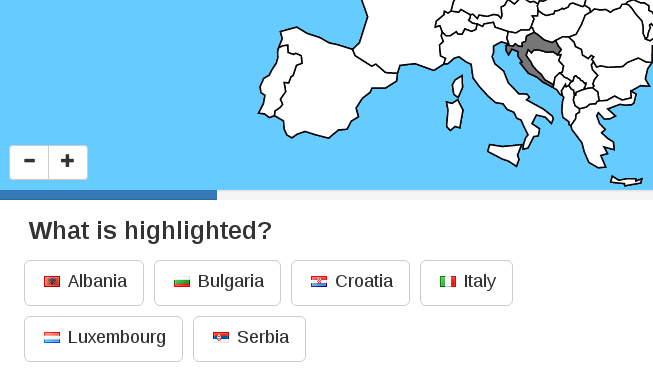
\includegraphics[height=4.5cm]{figures/question.png}
\end{frame}
% ------------------------------------------------------------------------------
% --------------------------- SLIDE --------------------------------------------
\begin{frame}
    \frametitle{Wrong answers}
    \centering
    \LARGE
    Problem in user interface

    \vfill
    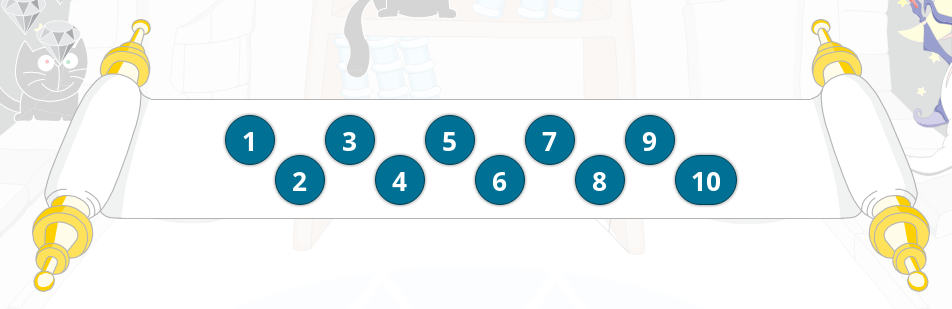
\includegraphics[width=\linewidth]{figures/keyboard.png}
\end{frame}
% ------------------------------------------------------------------------------
% --------------------------- SLIDE --------------------------------------------
\begin{frame}
    \frametitle{Wrong answers}
    \centering
    \LARGE
    \dots and much more
\end{frame}
% ------------------------------------------------------------------------------






% --------------------------- SLIDE --------------------------------------------
\begin{frame}
    \frametitle{Systems}
    \small
    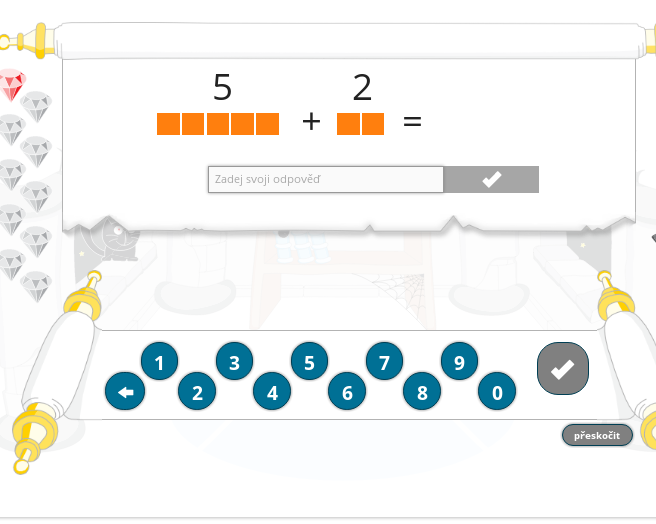
\includegraphics[height=2.5cm]{figures/matmat.png}
    \hfill
    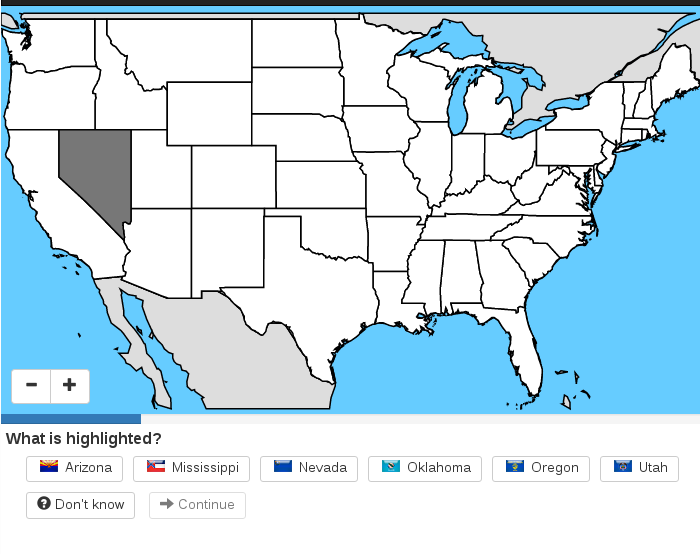
\includegraphics[height=2.5cm]{figures/slepemapy.png}
    \hfill
    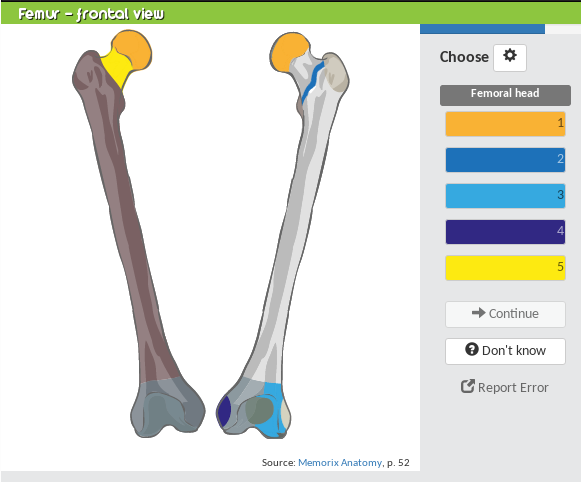
\includegraphics[height=2.5cm]{figures/anatom.png}

    \centering
    \begin{multicols}{3}
       \texttt{matmat.cz}

       \vspace{5mm}
       basic arithmetic

       \vspace{5mm}
       elementary school

    \columnbreak
       \texttt{outlinemaps.org}

       \vspace{5mm}
       geography

       \vspace{5mm}
       high school

    \columnbreak
       \texttt{practiceanatomy.com}

       \vspace{5mm}
       human anatomy

       \vspace{5mm}
       university
    \end{multicols}
\end{frame}
% ------------------------------------------------------------------------------
% --------------------------- SLIDE --------------------------------------------
\begin{frame}
    \frametitle{Systems}
    \small
    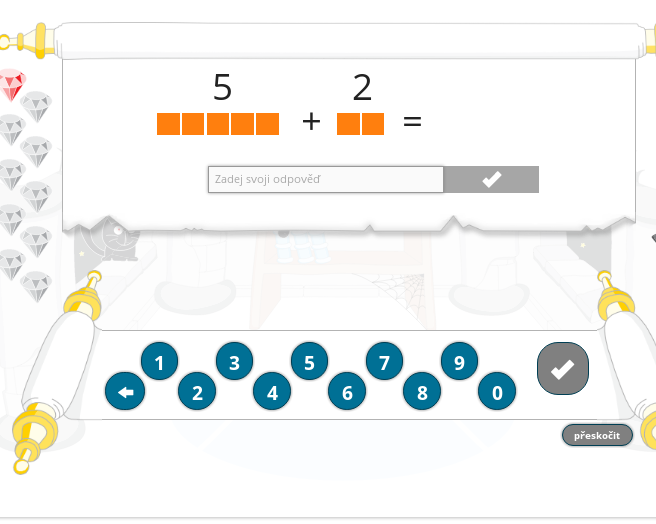
\includegraphics[height=2.5cm]{figures/matmat.png}
    \hfill
    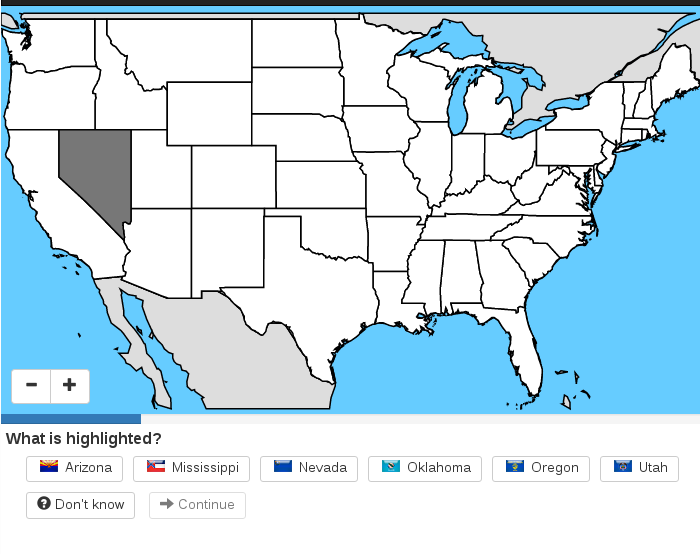
\includegraphics[height=2.5cm]{figures/slepemapy.png}
    \hfill
    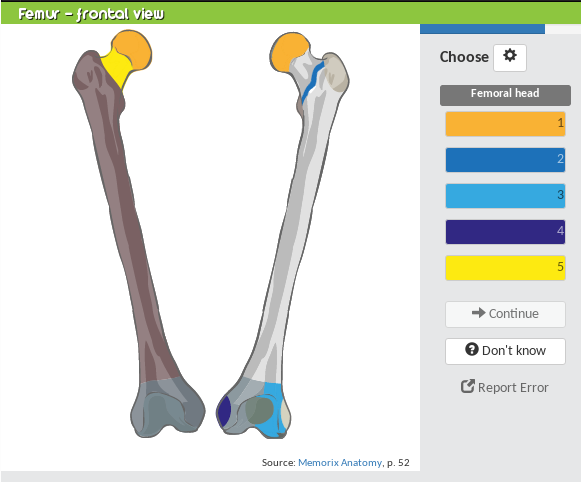
\includegraphics[height=2.5cm]{figures/anatom.png}

    \begin{itemize}
        \item simple tasks
        \item adaptivity - selection of questions
        \item $>$ \numprint{200000} answers
    \end{itemize}
\end{frame}
% ------------------------------------------------------------------------------
% --------------------------- SLIDE --------------------------------------------
\begin{frame}
    \centering
    \huge Wrong Answers - Geography
\end{frame}
% ------------------------------------------------------------------------------
% --------------------------- SLIDE --------------------------------------------
\begin{frame}
    \frametitle{Common Wrong Answers}
    \Large
    Countries
    \begin{itemize}
        \item common border, similar size, same first latter
        \item importance of practice context - Madagascar
    \end{itemize}
\end{frame}
% ------------------------------------------------------------------------------
% --------------------------- SLIDE --------------------------------------------
\begin{frame}
    \frametitle{Common Wrong Answers - Geography}
    \centering
    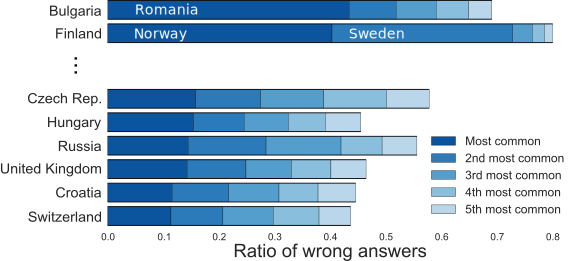
\includegraphics[width=\linewidth]{figures/wrong-answers-bar}
\end{frame}
% ------------------------------------------------------------------------------
% --------------------------- SLIDE --------------------------------------------
\begin{frame}
    \frametitle{Confusion Graph}
    \centering
    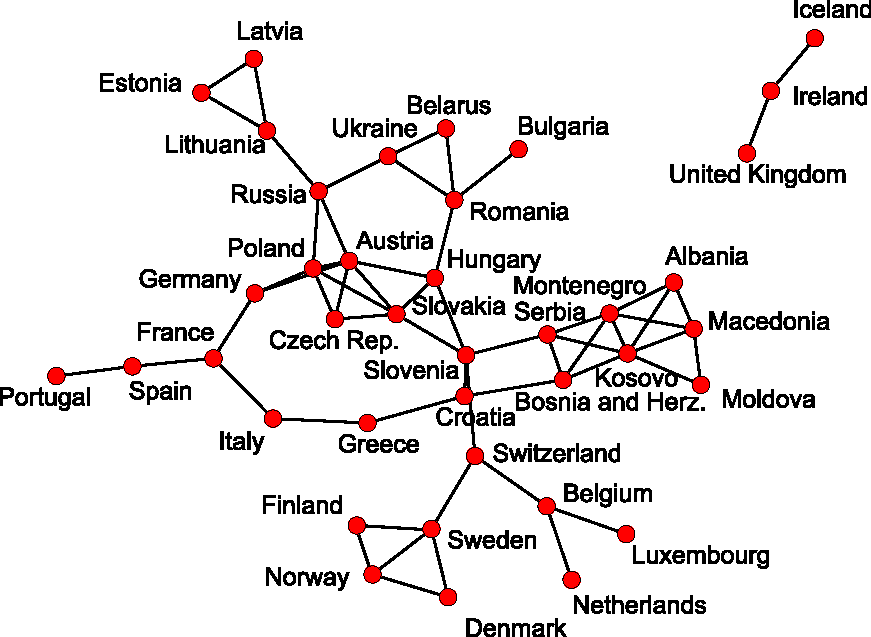
\includegraphics[width=\linewidth]{figures/confusion-clustering-graph}
\end{frame}
% ------------------------------------------------------------------------------
% --------------------------- SLIDE --------------------------------------------
\begin{frame}
    \frametitle{Item Clustering}
    \centering
    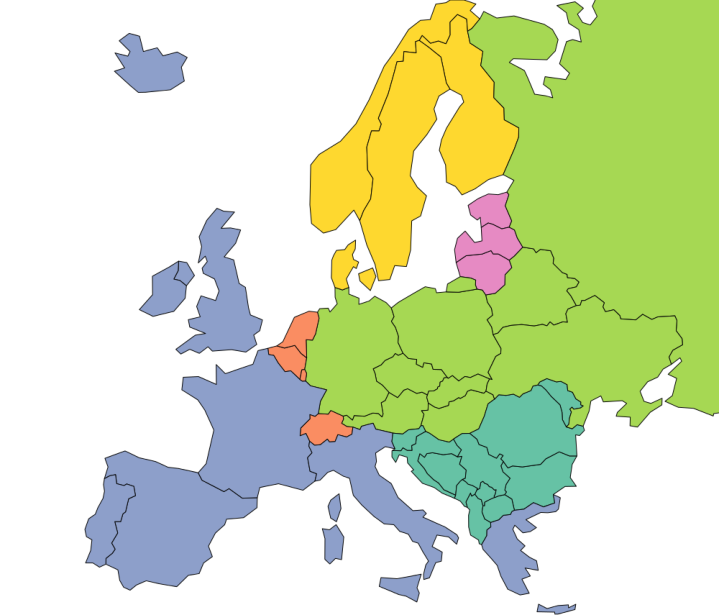
\includegraphics[width=0.7\linewidth]{figures/confusion-clustering-map}
\end{frame}
% ------------------------------------------------------------------------------



% --------------------------- SLIDE --------------------------------------------
\begin{frame}
    \centering
    \huge Cross-system Comparison
\end{frame}
% ------------------------------------------------------------------------------
% --------------------------- SLIDE --------------------------------------------
\begin{frame}
    \frametitle{Categories of Wrong Answers}
    \Large
    \begin{itemize}
        \item \textbf{TopWA} - most common wrong answer
        \item \textbf{CWA} - other common wrong answers - $> 5\%$
        \item \textbf{Other}
        \item \textbf{Missing} - question skipped by learner
    \end{itemize}
\end{frame}
% ------------------------------------------------------------------------------
% --------------------------- SLIDE --------------------------------------------
\begin{frame}
    \frametitle{System comparison}
    \centering
    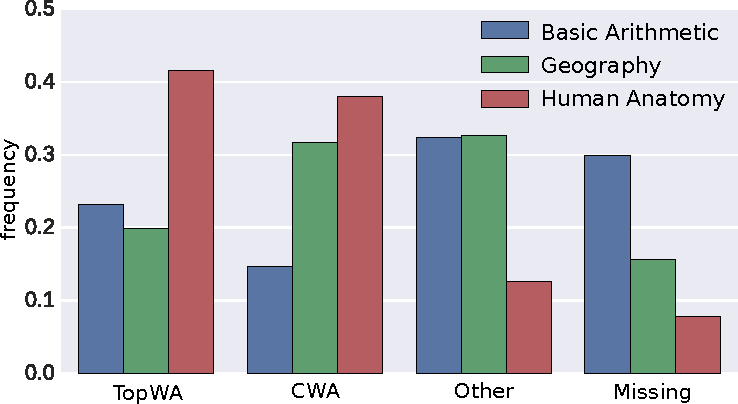
\includegraphics[width=\linewidth]{figures/system-comparison-distribution}
\end{frame}
% ------------------------------------------------------------------------------
% --------------------------- SLIDE --------------------------------------------
\begin{frame}
    \frametitle{System comparison - Response time}
    \centering
    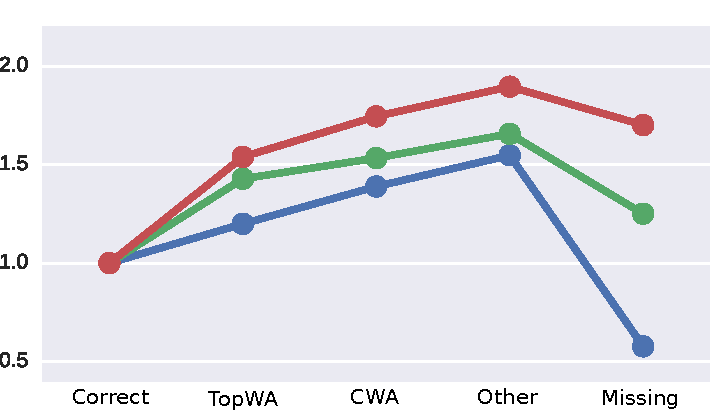
\includegraphics[width=0.8\linewidth]{figures/system-comparison-response-time}
\end{frame}
% ------------------------------------------------------------------------------
% --------------------------- SLIDE --------------------------------------------
\begin{frame}
    \frametitle{System comparison - Probability of Leaving}
    \centering
    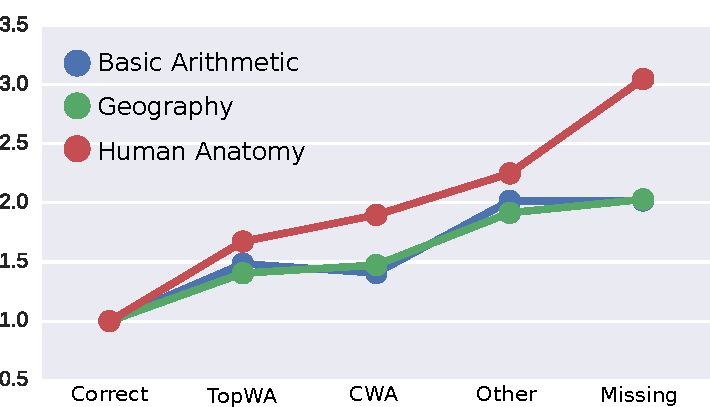
\includegraphics[width=0.8\linewidth]{figures/system-comparison-leaving}
\end{frame}
% ------------------------------------------------------------------------------
% --------------------------- SLIDE --------------------------------------------
\begin{frame}
    \frametitle{System comparison - Future Success}
    \centering
    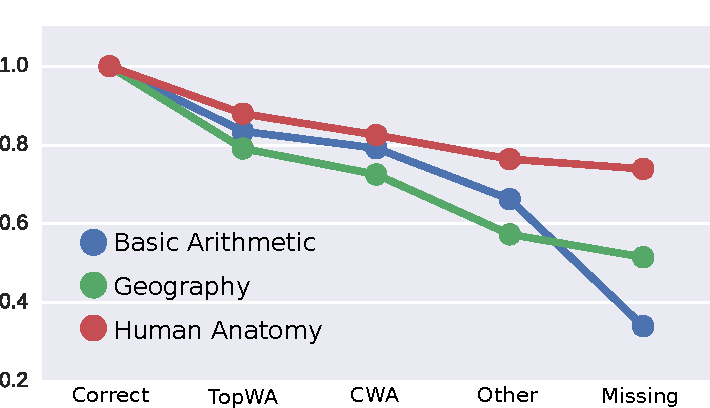
\includegraphics[width=0.8\linewidth]{figures/system-comparison-future-success}
\end{frame}
% ------------------------------------------------------------------------------
% --------------------------- SLIDE --------------------------------------------
\begin{frame}
    \frametitle{Categories of Wrong Answers}
    \Large
    \begin{itemize}
        \item \textbf{TopWA}, \textbf{CWA}, \textbf{Other}, \textbf{Missing}
        \item equally distributed
        \item linear behaviour
        \item similar behaviour in different domains
        \item good measure of wrongness - interval variable
    \end{itemize}
\end{frame}
% ------------------------------------------------------------------------------

% --------------------------- SLIDE --------------------------------------------
\begin{frame}
    \frametitle{Wrong Answers}
    \huge
    Wrong answers
    \Large
    \begin{itemize}
        \item are \textbf{easy to collect}
        \item has \textbf{many applications}: question and hint construction, feedback and inspiration, \dots
    \end{itemize}
    Contributions
    \begin{itemize}
        \item \textbf{item clustering}
        \item \textbf{measure of wrongness}
    \end{itemize}
\end{frame}
% ------------------------------------------------------------------------------

\end{document}
% ------------------------------------------------------------------------------
% ------------------------------------------------------------------------------
% ------------------------------------------------------------------------------
% --------------------------- SLIDE --------------------------------------------
\begin{frame}
    \frametitle{}
\end{frame}
% ------------------------------------------------------------------------------
\begin{itemize}
\end{itemize}
